% ===========================================================================
% chapters/mathematical_model.tex — Mathematical Model of the Isothermal
%                                   Tubular Reformer
% ===========================================================================

\chapter{Mathematical Model and Numerical Methods}\label{ch:reactor_model}

The previous two chapters established the building blocks. \Cref{ch:kinetic_model} fixed the lumped eight-reaction kinetic model that drives the chemistry; \cref{ch:governing_eqs} derived the convection-diffusion-reaction PDE~\eqref{eq:species_transport} and its finite-volume discretisation, ending at the per-cell semi-discrete \cref{eq:semidiscrete_full}. The present chapter pins those abstract objects to a specific physical reactor and then specifies how the resulting initial-value problem is solved numerically. \Crefrange{sec:isothermal}{sec:complete_system} fix the geometry, operating conditions, feed composition, side-stream injectors, and the few calibration choices that turn the formulation into a well-posed initial-value problem; \cref{sec:fortran,sec:solvers} then describe the implementation language and the three time-integration algorithms whose comparative performance is the subject of the next chapter.

The headline simplification carried throughout the model side of this chapter is the \emph{isothermal assumption} --- the reactor temperature is held at a single, uniform value and no enthalpy balance is solved. This decision is stated and defended in \cref{sec:isothermal}; its consequences propagate into the choice of dispersion coefficient (\cref{sec:Dax_dispersion}) and the activation-energy calibration of reaction~\eqref{eq:rxn5} retained from \cref{ssec:steam_reforming_benzene} of \cref{ch:kinetic_model}. The resulting model is best read as a benchmarking platform for the time-integration algorithms compared in the next chapter, not as a quantitative digital twin of an industrial reformer.

% ===========================================================================
% Use of Generative AI Models — unnumbered, per Saša's 2026-04-22 directive
% ===========================================================================

\section*{Use of Generative AI Models}\label{sec:ai_use}
\addcontentsline{toc}{section}{Use of Generative AI Models}

In compliance with the recommendation of the Department of Chemical Engineering and my supervisor, I declare the following regarding my use of generative artificial intelligence models in the preparation of this thesis. The single AI tool I used in the course of this work was Claude Code (Anthropic).

I used the tool for four kinds of task: review of the Fortran source code, grammar and spelling checks on the thesis text, generation of plotting scripts, and literature research. All model-level work remained with me --- including every model decision, the calibration choices documented later in this chapter, every numerical value reproduced in the thesis, the derivations of equations, and the interpretation of all results. I verified each output of the tool independently before incorporating it: I checked every literature citation against the original source via its DOI, I took every numerical value from the Fortran source of record, and my supervisor reviewed all chapters before submission. The full text of this thesis, including the literature review and the abstract, is my own work, as confirmed by the statement of authorship at the front of the document.

The AI tool was used in an editorial and exploratory capacity only; no model parameter, equation, numerical result, or interpretation reproduced in the following chapters originated from an AI tool without my independent verification.

% ===========================================================================
\section{Isothermal Assumption and Model Scope}\label{sec:isothermal}
% ===========================================================================

The temperature is held along the reactor at a single, uniform value
%
\begin{equation}
  T(x,t) \equiv T_{\mathrm{react}} = \SI{1173.15}{\kelvin}
  \quad (\approx \SI{900}{\degreeCelsius})
  \label{eq:isothermal_T}
\end{equation}
%
for every computational cell and every instant of the integration window. No enthalpy balance is solved alongside the species transport equations. Three considerations support this simplification at the present stage of the work. 

First, the primary objective of the thesis is to study the dynamic concentration evolution of a stiff reactive transport system and to benchmark candidate time-integration algorithms; isolating the chemistry from heat transfer keeps the numerical experiments interpretable. 

Second, an industrial reformer with a refractory liner and pre-heated feed approaches near-isothermal operation in its active conversion zone, so a uniform-\(T\) abstraction is a defensible first-cut model rather than an exotic choice. 

Third, decoupling chemistry from heat transfer is the standard pedagogical and prototyping starting point for tubular reactor modelling~\cite{Levenspiel1999, Fogler2006}. The isothermal assumption is not free of cost, and the chapter is honest about the price. 

Suppressing the energy balance propagates three concrete concessions through the model: one in how the rate constants are evaluated, one in how the cold reactant injectors are treated, and one in how the steam mass balance is closed. None of these are fatal in isolation, but each requires a downstream correction that this chapter has to declare openly.

(i)~I evaluate all eight Arrhenius rate constants once at the single reference temperature~\(T_{\mathrm{react}}\); the reaction source term~\(\Ri\) inherited from~\eqref{eq:species_transport} loses its \(T\)-dependence and reduces to a function of the local concentration vector alone.

(ii)~The cold side-stream injectors of oxygen and steam, which would physically enter at temperatures of order 300--500~\si{\kelvin} and locally depress the gas temperature, are introduced into a reactor that is everywhere at \SI{1173}{\kelvin}; the corresponding enthalpy sinks are ignored.

(iii)~With the steam-reforming reactions running at their full Arrhenius rate from the inlet rather than being Arrhenius-frozen by a cold inlet zone, the steam demand of the isothermal model exceeds the supply that would be reasonable for a non-isothermal reformer; this is addressed by enlarging the cell-1 \ce{H2O} injector, and the benzene steam-reforming reaction~\eqref{eq:rxn5} retains the calibrated activation energy \(E_5 = \SI{443}{\kilo\joule\per\mole}\) so that the soot-formation pathway can proceed at all.

A future extension that solves the energy balance alongside the species transport would remove both calibration choices identified above, since a cooler inlet zone naturally paces the steam-reforming reactions.

% ===========================================================================
\section{Reactor Geometry and Operating Conditions}\label{sec:geometry}
% ===========================================================================

I model the reactor as a straight cylindrical tube of length~\(L\) and constant internal diameter~\(d\), at uniform temperature~\(T_{\mathrm{react}}\) and total pressure~\(P\). I collect the geometric and operating parameters used throughout the simulations in \cref{tab:reactor_params}; they match the values hard-coded in the Fortran model that produces the simulation results of subsequent chapters.

\begin{table}[H]
\centering
\footnotesize
\caption{Reactor geometry and operating conditions; values match the Fortran model.}\label{tab:reactor_params}
\begin{tabular*}{\textwidth}{@{\extracolsep{\fill}}lll}
\toprule
Parameter & Symbol & Value \\
\midrule
Reactor length             & \(L\)            & \SI{20}{\metre} \\
Internal diameter          & \(d\)            & \SI{0.60}{\metre} \\
Cross-sectional area       & \(A = \pi d^2/4\)& \SI{0.2827}{\metre\squared} \\
Superficial gas velocity   & \(u\)            & \SI{0.516}{\metre\per\second} \\
Operating temperature      & \(T_{\mathrm{react}}\) & \SI{1173.15}{\kelvin} (\SI{900}{\degreeCelsius}) \\
Total pressure             & \(P\)            & \SI{101.325}{\kilo\pascal} \\
Number of finite volumes   & \(N\)            & 100 \\
Cell width                 & \(\Delta x = L/N\)& \SI{0.20}{\metre} \\
Axial dispersion coefficient   & \(\Dax\)     & \SI{1.0e-2}{\metre\squared\per\second}\(^{\ast}\) \\
\bottomrule
\end{tabular*}
\end{table}

The asterisk on~\(\Dax\) is unpacked in \cref{sec:Dax_dispersion}; the assumptions of \cref{sec:pfr_model} --- one-dimensional, axially symmetric, constant cross-section, approximately constant pressure --- all hold for these numbers. The mean residence time:
%
\begin{equation}
  \tau = \frac{L}{u} = \frac{20}{0.516} \approx \SI{38.8}{\second}
  \label{eq:residence_time}
\end{equation}
%
is the natural time-scale against which the integration window is calibrated. The runs reported in this chapter and the next use \(t_{\mathrm{end}} = \SI{50}{\second}\) --- slightly above one residence time --- which provides a comfortable margin past the front arrival to reach a stationary axial profile. A useful sanity check on the flow regime is the Reynolds number:
%
\begin{equation}
  \Re = \frac{u\,d}{\nu}
      = \frac{0.516 \times 0.60}{2.0\times 10^{-4}}
      \approx 1.55 \times 10^{3},
  \label{eq:reynolds_reactor}
\end{equation}
%
where \(\nu \approx \SI{2.0e-4}{\metre\squared\per\second}\) is representative for hot syngas at \SI{900}{\degreeCelsius}~\cite{Fogler2006}. The result places the flow just below the pipe-flow transition \(\Re \approx 2{,}300\), at the upper edge of the laminar regime; the implications for \(\Dax\) are unpacked in \cref{sec:Dax_dispersion}.

% ===========================================================================
\section{Feed Composition and Inlet Conditions}\label{sec:feed}
% ===========================================================================

\subsection{Species Tracked}\label{ssec:species_list}

I follow ten species in the simulation: three carbon-containing fuels (methane, benzene, an aromatic tar surrogate), the oxidant, two reforming products, the steam reactant, the soot product, and an inert diluent. They are listed in \cref{tab:species}; the index column \(i\) is the same index that appears in the state vector. I treat soot as a pseudo-gaseous species with an effective molar concentration, following the lumped approach of Jess~\cite{Jess1996}; nitrogen is purely a diluent and changes only through convective transport.

\begin{table}[H]
\centering
\footnotesize
\caption{Species tracked in the reactor model; indices follow the state-vector ordering of \cref{ssec:state_vector}.}\label{tab:species}
\begin{tabular*}{\textwidth}{@{\extracolsep{\fill}}clll}
\toprule
Index \(i\) & Species & Role in the model & Formula \\
\midrule
1  & Methane                  & Aliphatic surrogate         & \ce{CH4}   \\
2  & Benzene                  & Intermediate aromatic       & \ce{C6H6}  \\
3  & \(\alpha\)-Methylstyrene & Heavy tar surrogate         & \ce{C9H10} \\
4  & Oxygen                   & Oxidant (injected only)     & \ce{O2}    \\
5  & Carbon monoxide          & Partial-oxidation product   & \ce{CO}    \\
6  & Hydrogen                 & Product / R5 inhibitor      & \ce{H2}    \\
7  & Steam                    & Reforming agent (injected)  & \ce{H2O}   \\
8  & Carbon dioxide           & Steam-reforming product     & \ce{CO2}   \\
9  & Soot (carbon)            & Solid product               & \ce{C}     \\
10 & Nitrogen                 & Inert diluent               & \ce{N2}    \\
\bottomrule
\end{tabular*}
\end{table}

\subsection{Inlet Mole Fractions and Concentration Conversion}\label{ssec:inlet}

The full inlet composition is given in \cref{tab:inlet_composition}. At the reactor inlet, the gas is a model pyrolytic mixture dominated by the heavy aromatic surrogate and methane, with smaller contributions of hydrogen, carbon monoxide, and carbon dioxide; the oxygen and water that drive the partial-oxidation and steam-reforming chemistry are deliberately absent and enter only through the side-stream injectors. The inlet mole fractions are converted to molar concentrations via the ideal-gas law at the reactor temperature and pressure. The total molar concentration is
%
\begin{equation}
  C_{\mathrm{tot}}
  = \frac{P}{R\,T_{\mathrm{react}}}
  = \frac{\SI{101325}{\pascal}}{\SI{8.314}{\joule\per\mole\per\kelvin}\times\SI{1173.15}{\kelvin}}
  \approx \SI{10.4}{\mole\per\metre\cubed},
  \label{eq:ideal_gas_total}
\end{equation}
%
and the inlet concentration of species~\(i\) is
%
\begin{equation}
  C_{i,\mathrm{in}} = y_{i,\mathrm{in}}\,C_{\mathrm{tot}}.
  \label{eq:inlet_conc}
\end{equation}
%
\begin{table}[!t]
\centering
\footnotesize
\caption{Inlet mole fractions of the model pyrolytic gas. Unlisted species enter at zero; \ce{O2} and \ce{H2O} arrive through the side-stream injectors of \cref{sec:injectors}.}\label{tab:inlet_composition}
\begin{tabular*}{\textwidth}{@{\extracolsep{\fill}}clr}
\toprule
Index \(i\) & Species & Mole fraction \(y_{i,\mathrm{in}}\) \\
\midrule
1  & \ce{CH4}   & 0.51382 \\
3  & \ce{C9H10} & 0.39711 \\
6  & \ce{H2}    & 0.06714 \\
5  & \ce{CO}    & 0.01141 \\
8  & \ce{CO2}   & 0.01053 \\
\bottomrule
\end{tabular*}
\end{table}
%
The vector \(\Cin\) defined in this way is the concrete realisation of the inlet vector that appears in the Dirichlet condition~\eqref{eq:dirichlet_inlet} of \cref{ch:governing_eqs}, completing the specification of the feed in concentration form. The single parameter in \cref{tab:reactor_params} that still requires physical justification is the axial dispersion coefficient~\(\Dax\), whose value lies at the boundary between the laminar and transitional regimes; its derivation is the subject of the next section.
% ===========================================================================
\section{Axial Dispersion: Laminar--Turbulent Regime}\label{sec:Dax_dispersion}
% ===========================================================================

I choose \(\Dax\) carefully because the operating conditions sit at the boundary between the laminar regime, where the classical Aris-Taylor formula~\eqref{eq:aris_taylor} applies, and the transitional regime, where empirical turbulent-pipe correlations take over. Neither limit is unambiguously appropriate; the value I report in \cref{tab:reactor_params} comes from the empirical correlation, with its limits and assumptions stated openly. A laminar Aris-Taylor estimate~\cite{Taylor1953, Aris1956}, with molecular diffusivity \(D_{AB} \approx \SI{2e-4}{\metre\squared\per\second}\) for light gases at \SI{900}{\degreeCelsius}~\cite{Fogler2006} and the geometry of \cref{tab:reactor_params} (\(u = \SI{0.516}{\metre\per\second}\), tube radius \(R = d/2 = \SI{0.30}{\metre}\)), gives
%
\begin{equation*}
  \Dax^{\mathrm{Aris-Taylor}}
  = D_{AB} + \frac{u^2 R^2}{48\,D_{AB}}
  \approx 2\times 10^{-4} + \frac{(0.516)^2 (0.30)^2}{48\times 2\times 10^{-4}}
  \approx \SI{2.5}{\metre\squared\per\second}.
\end{equation*}
%
This estimate rests on the assumption of a fully developed laminar parabolic profile, which is violated for the present reactor on three counts: the side-injection ports introduce strong cross-sectional concentration gradients near each injector cell; the axial density variation produced by reactions~\eqref{eq:rxn1}--\eqref{eq:rxn8} (mean molar mass falling from \(\overline{M}\approx\SI{56}{\gram\per\mol}\) at the inlet to \(\overline{M}\approx\SI{30}{\gram\per\mol}\) once steam reforming has converted the heavy hydrocarbons) breaks the constant-property assumption; and the Reynolds number of \cref{eq:reynolds_reactor} sits at the upper edge of the laminar band, so any of these perturbations can plausibly trip the flow into transitional behaviour. The Aris-Taylor formula is therefore an upper bound, not a defensible point estimate. A more appropriate framework for this regime is the empirical correlation of axial dispersion in turbulent pipe flow reported by Levenspiel~\cite{Levenspiel1999}. He reports the dimensionless Bodenstein number \(\mathrm{Pe}_d = u\,d/\Dax\) in the band \(1\)--\(10\) for \(\Re\) between roughly~\(2{,}000\) and~\(10{,}000\), with the lower edge of that band corresponding to flows near the laminar transition. The present operating point at \(\Re \approx 1{,}550\) lies just below the calibration range of this correlation: a direct extrapolation toward lower \(\Re\) would push \(\mathrm{Pe}_d\) further down (i.e.\ \(\Dax\) further up), in the same direction as the laminar Aris-Taylor estimate above. I therefore depart from a strict application of the correlation and adopt \(\mathrm{Pe}_d \approx 30\), several times below the \(\Dax\) the correlation would predict at fully developed turbulent conditions, giving
%
\begin{equation*}
  \Dax = \frac{u\,d}{\mathrm{Pe}_d}
       = \frac{0.516 \times 0.60}{30}
       \approx \SI{1.0e-2}{\metre\squared\per\second},
\end{equation*}
%
which is the value listed in \cref{tab:reactor_params}. The remaining sanity checks on this choice are the global P\'eclet number for the full reactor length
%
\begin{equation}
  \Pe = \frac{u\,L}{\Dax}
      = \frac{0.516 \times 20}{10^{-2}}
      \approx 1{,}032,
  \label{eq:pe_reactor}
\end{equation}
%
which keeps the reactor strongly convection-dominated, and the cell P\'eclet number on the uniform grid of \cref{tab:reactor_params}
%
\begin{equation}
  \Pe_{\mathrm{cell}}
  = \frac{u\,\Delta x}{\Dax}
  = \frac{0.516 \times 0.20}{10^{-2}}
  \approx 10,
  \label{eq:pe_cell}
\end{equation}
%
which is well above the central-differencing stability threshold of~2. The first-order upwind scheme of \cref{eq:upwind} is therefore the appropriate choice for the convective flux. A complementary characteristic length is the Taylor smearing distance accumulated over the residence time of \cref{eq:residence_time},
%
\begin{equation*}
  \sigma = \sqrt{2\Dax\,\tau} \approx \SI{0.88}{\metre},
\end{equation*}
%
about four cells, which is small enough to preserve the cell-1 front-loaded steam profile, and large enough that the dispersion contribution to the system Jacobian is non-trivial and improves the conditioning of the implicit time-integration solvers compared with the pure-PFR limit \(\Dax \to 0\). Substituting the Aris-Taylor value \(\Dax \approx \SI{2.5}{\metre\squared\per\second}\) directly into the isothermal model was confirmed empirically to break the chemistry: at \(\Pe \approx 4\) the reactor enters the diffusion-dominated regime, the cell-1 \ce{H2O} boost smears across the whole reactor within one residence time, and the steam-reforming reactions shut off under the \(\max(\bar{C}_{i,j}, 0)\) clamp. The isothermal assumption combined with fully laminar dispersion has no operating point at which the chemistry both runs to completion and conserves steam; the proper resolution is the energy-balance extension of \cref{sec:isothermal}.

% ===========================================================================
\section{Side-Injection Model for Oxygen and Steam}\label{sec:injectors}
% ===========================================================================

\subsection{Physical Motivation}\label{ssec:injector_motivation}

The pyrolytic gas entering the reactor is dry: oxygen and water are absent from the inlet stream listed in \cref{tab:inlet_composition}. Both reactants are introduced through nine discrete side-stream injectors, but with rather different axial distributions. 

Oxygen is staged along the length of the reactor: it sustains the partial-oxidation reactions~\eqref{eq:rxn1}--\eqref{eq:rxn3} past the initial inlet zone, where they would otherwise be quenched by oxygen depletion, and the staged supply mimics the feed design used in industrial reformers to control hot-spot formation and to extend the active reaction zone. Steam, by contrast, is overwhelmingly concentrated at the inlet (cell~1), with the eight downstream injectors providing only top-up amounts. 

This front-loaded layout closes the isothermal steam mass balance --- the third concession identified in \cref{sec:isothermal} --- and is reflected in the cell-1 \ce{H2O} flow rate of \cref{tab:injectors}. Steam itself drives the reforming reactions~\eqref{eq:rxn4}--\eqref{eq:rxn6} and the soot gasification of \cref{eq:rxn8}.

\subsection{Logical-Switch Source Term}\label{ssec:logical_switch}

In the finite-volume framework of \cref{ch:governing_eqs}, each injector is modelled as a point source localised to a single computational cell. Following the design pattern proposed by the supervisor, every cell formally carries an injector slot for every species, but the slot contributes only when a logical switch is on. 

Consider \(K\) injectors, with the \(k\)-th delivering molar flow \(\dot{n}_{i,\mathrm{inj}}^{(k)}\) [\si{\mole\per\second}] of species~\(i\) into cell \(j_{\mathrm{inj}}^{(k)}\). Distributing each injection uniformly over its cell volume \(V_{\mathrm{cell}} = A\,\Delta x\) and summing over all injectors gives the volumetric source \(S_{\mathrm{i,j}}\) where the Kronecker delta selects only the host cell of each injector. The result has units of \si{\mole\per\metre\cubed\per\second}, matching the reaction source~\(R_i\) inherited from~\eqref{eq:species_transport}.
%
\begin{equation}
  S_{i,j}
  = \sum_{k=1}^{K} \frac{\dot{n}_{i,\mathrm{inj}}^{(k)}}{A\,\Delta x}\,
    \delta_{j,\,j_{\mathrm{inj}}^{(k)}},
  \label{eq:injection_total}
\end{equation}
%


\subsection{Injector Locations and Flow Rates}\label{ssec:injector_table}

\begin{figure}[H]
\centering
\resizebox{\textwidth}{!}{%
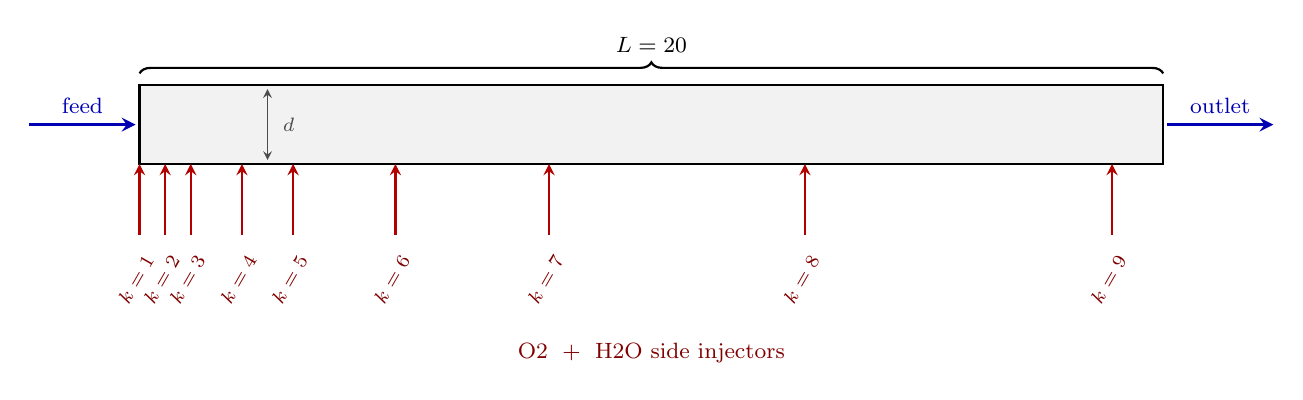
\begin{tikzpicture}[>=stealth, thick, every node/.style={font=\small}]
  % Drawing scale: 1 m of reactor -> \Lscale cm of drawing width
  \def\Lscale{0.65}
  % Reactor tube
  \draw[thick, fill=gray!10]
    (0, 0) rectangle (\Lscale*20, 1.0);
  % Inlet feed arrow
  \draw[->, very thick, blue!70!black]
    (-1.4, 0.5) -- (-0.05, 0.5)
    node[midway, above, font=\footnotesize] {feed};
  % Outlet arrow
  \draw[->, very thick, blue!70!black]
    (\Lscale*20+0.05, 0.5) -- (\Lscale*20+1.4, 0.5)
    node[midway, above, font=\footnotesize] {outlet};
  % Injector arrows with rotated labels to avoid collision in the dense inlet zone
  \foreach \pos/\k in {0/1, 0.5/2, 1/3, 2/4, 3/5, 5/6, 8/7, 13/8, 19/9} {
    \draw[->, red!70!black, thick]
      (\Lscale*\pos, -0.9) -- (\Lscale*\pos, 0);
    \node[font=\scriptsize, red!50!black, rotate=60, anchor=north east]
      at (\Lscale*\pos, -0.95) {\(k=\k\)};
  }
  % Injection species label centered below
  \node[font=\footnotesize, red!50!black]
    at (\Lscale*10, -2.4) {\ce{O2} \;+\; \ce{H2O} side injectors};
  % Length annotation
  \draw[decorate, decoration={brace, mirror, amplitude=4pt}]
    (\Lscale*20, 1.15) -- (0, 1.15)
    node[midway, above=4pt, font=\footnotesize] {\(L = \SI{20}{\metre}\)};
  % Diameter annotation inside reactor between injectors 4 and 5 (per Saša 2026-05-17)
  \draw[<->, gray!60!black, thin]
    (\Lscale*2.5, 0.05) -- (\Lscale*2.5, 0.95)
    node[pos=0.5, right=2pt, font=\scriptsize, gray!60!black] {\(d\)};
\end{tikzpicture}%
}
\caption{Schematic of the isothermal tubular reformer (not to scale). Nine side-stream injectors, indexed \(k = 1, \ldots, 9\), introduce oxygen and steam at axial positions given in \cref{tab:injectors}.}%
\label{fig:reactor_schematic}
\end{figure}

Nine injection ports are distributed along the reactor axis. The cell indices are obtained by mapping each axial position onto the uniform grid of cell centres \(x_j = (j - \tfrac{1}{2})\,\Delta x\) with \(\Delta x = \SI{0.20}{\metre}\), giving the index sequence \(j_{\mathrm{inj}}^{(k)} \in \{1, 3, 5, 10, 15, 25, 40, 65, 95\}\). The first three ports cluster within the first metre of the reactor: they sustain partial oxidation through the inlet zone (oxygen) and pre-load the steam reservoir for the steam-reforming reactions that begin immediately at \(T_{\mathrm{react}}\) (water). The downstream ports thin out toward the outlet, reflecting the diminishing demand once the aromatic load has been largely converted. \Cref{fig:reactor_schematic} shows the layout schematically; the numerical values of all nine injectors are listed in \cref{tab:injectors}.

\begin{table}[H]
\centering
\footnotesize
\caption{Side-stream injector positions and molar flow rates. Cell-1 water is enlarged to \SI{6.0}{\mole\per\second} (reference \SI{0.166}{\mole\per\second}) to close the isothermal steam balance.}\label{tab:injectors}
\begin{tabular*}{\textwidth}{@{\extracolsep{\fill}}cccrr}
\toprule
\(k\) & Position [m] & Cell \(j_{\mathrm{inj}}^{(k)}\) &
  \(\dot{n}_{\mathrm{O_2}}^{(k)}\) [\si{\mole\per\second}] &
  \(\dot{n}_{\mathrm{H_2O}}^{(k)}\) [\si{\mole\per\second}] \\
\midrule
1 & 0.0  & 1  & 0.205 & \textbf{6.000} \\
2 & 0.5  & 3  & 0.240 & 0.590 \\
3 & 1.0  & 5  & 0.200 & 0.560 \\
4 & 2.0  & 10 & 0.210 & 0.430 \\
5 & 3.0  & 15 & 0.170 & 0.390 \\
6 & 5.0  & 25 & 0.180 & 0.240 \\
7 & 8.0  & 40 & 0.160 & 0.060 \\
8 & 13.0 & 65 & 0.150 & 0.010 \\
9 & 19.0 & 95 & 0.160 & 1\,\(\times 10^{-6}\) \\
\midrule
  & Total & & 1.675 & 8.280 \\
\bottomrule
\end{tabular*}
\end{table}
\FloatBarrier

% ===========================================================================
\needspace{8\baselineskip}% keep \section{} from orphaning above its first \subsection
\section{Complete Semi-Discrete ODE System}\label{sec:complete_system}
% ===========================================================================

\subsection{Governing ODE per Cell}\label{ssec:per_cell_ode}

Specialising the per-cell semi-discrete \cref{eq:semidiscrete_full} of \cref{ch:governing_eqs} by adding the injection source term~\eqref{eq:injection_total}, the governing ordinary differential equation for species~\(i\) in cell~\(j\) becomes
%
\begin{equation}
  \frac{\mathrm{d}\bar{C}_{i,j}}{\mathrm{d}t}
  = \underbrace{-\,u\,\frac{\bar{C}_{i,j} - \bar{C}_{i,j-1}}{\Delta x}}_{\text{convection}}
  \;+\; \underbrace{\Dax\,\frac{\bar{C}_{i,j+1} - 2\,\bar{C}_{i,j} + \bar{C}_{i,j-1}}{(\Delta x)^{2}}}_{\text{diffusion}}
  \;+\; \underbrace{R_i(\bar{\vect{C}}_j)}_{\text{reaction}}
  \;+\; \underbrace{S_{i,j}}_{\text{injection}},
  \label{eq:full_per_cell}
\end{equation}
%
for \(j = 1, \ldots, N\) and \(i = 1, \ldots, N_s\). The reaction term~\(R_i(\bar{\vect{C}}_j)\) carries no explicit temperature dependence here, as a direct consequence of the isothermal assumption~\eqref{eq:isothermal_T}: the rate constants are evaluated once at \(T_{\mathrm{react}}\) using the Arrhenius parameters of \cref{ch:kinetic_model}. The boundary treatment is inherited unchanged from \cref{ssec:semidiscrete_ode}: a Dirichlet ghost cell \(\bar{C}_{i,0} = C_{i,\mathrm{in}}\) at the inlet and a zero-gradient ghost cell \(\bar{C}_{i,N+1} = \bar{C}_{i,N}\) at the outlet, so \cref{eq:full_per_cell} applies uniformly across all cells.

\subsection{State Vector and System Dimension}\label{ssec:state_vector}

All cell-averaged concentrations are stacked into a single state vector \(\vect{y}(t)\) of dimension \(N_s \times N\). The Fortran model uses a \emph{cell-grouped, species-fastest} ordering, in which the species index \(i\) varies fastest within each cell block:
%
\begin{equation}
  y_{(j-1)\,N_s + i}(t) = \bar{C}_{i,j}(t),
  \qquad i = 1, \ldots, N_s,
  \;\; j = 1, \ldots, N.
  \label{eq:state_vector_ordering}
\end{equation}
%
With \(N_s = 10\) species and \(N = 100\) cells, the state vector contains \(1{,}000\) unknowns. The cell-grouped ordering keeps the data accessed by the finite-volume stencil contiguous in memory --- evaluating the right-hand side of \cref{eq:full_per_cell} for cell~\(j\) touches three consecutive blocks of ten doubles --- which is the natural choice for the stencil-driven RHS assembly of the model.

Collecting the per-cell equations~\eqref{eq:full_per_cell} into vector form gives the compact system
%
\begin{equation}
  \frac{\mathrm{d}\vect{y}}{\mathrm{d}t}
  = \vect{f}_{\mathrm{conv}}(\vect{y})
  + \vect{f}_{\mathrm{diff}}(\vect{y})
  + \vect{f}_{\mathrm{rxn}}(\vect{y})
  + \vect{s},
  \label{eq:ode_split}
\end{equation}
%
where the four terms collect the convective, diffusive, reactive, and injection contributions respectively. The injection vector~\(\vect{s}\) is constant in time and depends on neither~\(\vect{y}\) nor~\(t\), so it does not contribute to the Jacobian \(\vect{J} = \partial \vect{f}/\partial \vect{y}\); the block-banded sparsity pattern of \(\vect{J}\) discussed in \cref{ssec:semidiscrete_ode} is therefore preserved unchanged.

The initial condition adopted in this work is a vacuum,
%
\begin{equation}
  \bar{C}_{i,j}(0) = 0
  \quad\text{for all}\quad i = 1, \ldots, N_s,\; j = 1, \ldots, N.
  \label{eq:ic_vacuum}
\end{equation}
%
This represents an empty reactor at \(t = 0\), when feed and side-stream injectors are switched on. The vacuum start avoids an artefact of the uniform-feed alternative \(\bar{C}_{i,j}(0) = C_{i,\mathrm{in}}\), which would place \ce{C9H10} at its inlet value in every cell and trigger reaction~\eqref{eq:rxn6} on non-existent steam before the cell-1 wavefront arrives. A startup transient of roughly \(\tau\) follows, after which the steady state is established; alternative initial conditions (uniform feed, \ce{N2}-purged, steam-purged) give the same steady state.

% ===========================================================================
\section{Choice of Implementation Language}\label{sec:fortran}
% ===========================================================================

The simulation reported in this thesis is implemented in Fortran. The choice was made on my supervisor's recommendation, motivated by Fortran's well-documented performance advantage on arithmetic-heavy numerical workloads: benchmarks consistently place ahead-of-time compiled languages in the top tier and interpreted alternatives such as Python one to two orders of magnitude behind~\cite{Pereira2017}. This advantage matters specifically for the present work, where the same right-hand-side function is evaluated under three different time-integration algorithms; any per-call overhead introduced by a slower runtime would pollute the wall-clock measurements and make the comparison reflect the language environment rather than the algorithms themselves. Fortran (\emph{Formula Translation}) was developed at IBM by John Backus and his team and first published in 1957~\cite{Backus1957} with the explicit objective of producing a high-level language whose compiler would emit machine code competitive with hand-written assembly for scientific calculations; almost seven decades of refinement have followed~\cite{MetcalfReidCohen2018}, all aimed at tight loops over arrays of numbers. The performance follows from two design choices: ahead-of-time compilation, which translates the source into the exact CPU instructions before the program runs --- where Python and MATLAB translate each line on the fly, roughly the difference between reading a book already translated and listening to a live interpreter at a conference; and automatic vectorisation, where the compiler safely emits CPU instructions that perform several arithmetic operations per clock cycle on ordinary loops, while higher-level languages reach this level only through compiled libraries, with per-call overhead that dominates on small per-cell arrays. The same algorithm therefore completes in seconds where equivalent Python or MATLAB code would take minutes, and the wall-clock differences reported in the next chapter reflect the algorithms themselves, not the language.

% ===========================================================================
\section{Time-Integration Algorithms}\label{sec:solvers}
% ===========================================================================

Three time-integration algorithms are implemented and benchmarked, each representing one canonical strategy: forward Euler, an explicit fixed-step method; backward Euler with a banded Newton iteration, an implicit fixed-step method; and the variable-step, variable-order backward differentiation formula (BDF) family in DLSODE~\cite{Hindmarsh1983}, an adaptive method-of-lines solver. All three operate on the same right-hand side~\(\vect{f}\) of \cref{eq:ode_split} and differ only in their internal step structure.

\subsection{Forward Euler}\label{ssec:forward_euler}

The forward Euler scheme advances the state by the explicit update
\begin{equation}
  \vect{y}_{n+1} = \vect{y}_n + \Delta t\,\vect{f}(\vect{y}_n),
  \label{eq:fwd_euler}
\end{equation}
costing one right-hand-side evaluation per step and yielding first-order accuracy in time. The method is only conditionally stable; for the convection-diffusion-reaction discretisation of \cref{ch:governing_eqs} the dominant restriction is the Courant--Friedrichs--Lewy (CFL) condition
\begin{equation}
  \Delta t \;<\; \frac{\Delta x}{u},
  \label{eq:cfl}
\end{equation}
which evaluates to \(\Delta t < \SI{0.39}{\second}\) at the standard configuration of \cref{tab:reactor_params}. The reactive source term~\(R_i\) imposes a secondary stability bound through the largest Arrhenius rate constant, but at \(T_{\mathrm{react}} = \SI{1173}{\kelvin}\) the chemical timescales remain well above the convective limit and the CFL constraint is the binding one.

The default integration step adopted here is \(\Delta t = \SI{1}{\milli\second}\), three orders of magnitude below the CFL bound. A divergence guard aborts the integration whenever any state component exceeds \(10^{15}\) in magnitude or becomes non-finite; the safety net is exercised in the next chapter, where pushing \(\Delta t\) past the CFL limit produces a numerical blow-up.

\subsection{Backward Euler with Banded Newton}\label{ssec:backward_euler}

The implicit counterpart of \cref{eq:fwd_euler} is the backward Euler step
\begin{equation}
  \vect{y}_{n+1} = \vect{y}_n + \Delta t\,\vect{f}(\vect{y}_{n+1}),
  \label{eq:bwd_euler}
\end{equation}
in which the right-hand side is evaluated at the unknown end-of-step state. The method is unconditionally A-stable for any step size~\(\Delta t > 0\), removing the CFL restriction at the price of the necessity of solving a generally nonlinear algebraic system at every integration step.

Solving \cref{eq:bwd_euler} for \(\vect{y}_{n+1}\) is cast as the residual root-finding problem
\begin{equation}
  \vect{g}(\vect{y}_{n+1}) \;=\; \vect{y}_{n+1} - \vect{y}_n - \Delta t\,\vect{f}(\vect{y}_{n+1}) \;=\; \vect{0},
  \label{eq:newton_residual}
\end{equation}
solved by Newton iteration. The Newton update reads
\begin{equation*}
  \vect{J}\,\bm{\delta} = -\vect{g}(\vect{y}^{(k)}), \qquad \vect{y}^{(k+1)} = \vect{y}^{(k)} + \bm{\delta},
\end{equation*}
with iteration Jacobian
\begin{equation*}
  \vect{J} \;=\; \frac{\partial \vect{g}}{\partial \vect{y}} \;=\; \vect{I} - \Delta t\,\frac{\partial \vect{f}}{\partial \vect{y}}
\end{equation*}
constructed by finite differences. The matrix \(\partial\vect{f}/\partial\vect{y}\) inherits the block-banded sparsity pattern of \cref{ssec:state_vector}, with lower and upper half-bandwidths \(\mathrm{ML} = \mathrm{MU} = N_s = 10\).

Curtis--Powell--Reid colouring~\cite{Curtis1974} exploits this band structure: because each column of the Jacobian affects only a narrow strip of rows, columns at sufficient distance from each other can be perturbed simultaneously without their effects overlapping. The number of right-hand-side evaluations needed to assemble the full Jacobian is therefore \(\mathrm{ML} + \mathrm{MU} + 1 = 21\) rather than \(N_{\mathrm{eqs}} = 1{,}000\). The factorisation is performed by the LINPACK banded LU routines bundled with ODEPACK; for the present bandwidth, the per-factor cost drops from \(\mathcal{O}(N_{\mathrm{eqs}}^{3})\) for a dense system to \(\mathcal{O}(\mathrm{ML}\cdot\mathrm{MU}\cdot N_{\mathrm{eqs}})\), a factor of approximately \(2{,}300\) on the standard grid.

At each integration step the Newton iteration is initialised at \(\vect{y}^{(0)} = \vect{y}_n\); the Jacobian is built and factored once at this initial guess, and the factorisation is reused for subsequent corrections. Convergence is declared when \(\lVert\bm{\delta}\rVert_\infty\) falls below a relative tolerance of \(10^{-6}\). If two successive corrections fail to halve in magnitude the Jacobian is rebuilt at the current iterate, on the assumption that the cached factorisation no longer represents the local landscape; the iteration is capped at twenty Newton steps to guarantee a graceful abort on non-convergent inputs. At the default step size \(\Delta t = \SI{10}{\milli\second}\), Newton converges in two to three steps over most of the trajectory, with one Jacobian build per integration step in the smooth regime and an occasional rebuild during the inlet startup transient.

\subsection{Method of Lines via DLSODE}\label{ssec:lsoda}

In contrast to the fully discrete schemes of \cref{ssec:forward_euler,ssec:backward_euler}, where the time variable is collapsed onto a fixed-step recurrence at the user's prescription, the method of lines treats the spatial discretisation and the time integration as separate concerns: the semi-discrete ODE system of \cref{eq:ode_split} is handed to a general-purpose ODE solver that selects its own internal time discretisation adaptively. The integrator used in this work is DLSODE from the ODEPACK library~\cite{Hindmarsh1983}, a stiff ODE solver based on the backward differentiation formulae (BDF) of orders one through five --- linear multistep schemes that combine several past states in the implicit relation
\begin{equation*}
  \sum_{j=0}^{k}\alpha_j\,\vect{y}_{n+1-j} = \Delta t\,\beta_0\,\vect{f}(\vect{y}_{n+1}),
\end{equation*}
of which backward Euler (\(k = 1\)) is the simplest case. As in \cref{ssec:backward_euler}, the implicit step is solved by a Newton iteration, but DLSODE caches and reuses the factored Jacobian across multiple steps until convergence quality degrades, amortising the dominant cost of stiff integration. DLSODE is configured here with method flag \(\mathrm{mf} = 25\), which selects the BDF family with an internally generated banded finite-difference Jacobian whose half-bandwidths match the FVM stencil, \(\mathrm{ML} = \mathrm{MU} = N_s\). Local error tolerances are set to \(10^{-5}\) relative and \(10^{-9}\) absolute.

Two adaptive mechanisms distinguish DLSODE from the fixed-step backward Euler scheme of \cref{ssec:backward_euler}. First, the step size~\(\Delta t\) is selected at every internal step from a local truncation error estimate based on the predictor--corrector difference: it grows where the solution is smooth and contracts automatically as the inlet transient injects sharp fronts into the reactor. Second, the BDF order~\(k\) varies between one and five under the same work-per-accuracy heuristic, with higher~\(k\) yielding smaller truncation error per step at the price of more state history. 

On the present problem the order typically escalates to BDF-3 or BDF-4 once the inlet transient has decayed, and the total internal step count over the \SI{50}{\second} integration window ranges from approximately one hundred at the coarsest grid to over one thousand at the finest. These adaptive mechanisms remove the need for hand-tuned step sizing and provide a documented level of local accuracy; they are also the source of the per-step overhead that the comparison in the next chapter quantifies.

